\newpage
\section{Appendixes}
% \begin{table}[h]
% %\centering
% \begin{tabular}{ p{2.3cm} p{2.3cm} p{2cm}}
%  \toprule
%  Features&&\\
%  \midrule
%  sex&age\_cat&race  \\
%  juv\_fel\_count&juv\_misd\_count&juv\_other\_count\\
%  priors\_count&c\_charge\_degree&is\_recid\\[0.5pt]
%  score\_text \\
%   \bottomrule
% \end{tabular}
% \caption{}
%     \label{high_compas_features}
% \end{table}

% \begin{table}[h]
% %\centering
% \begin{tabular}{ p{0.3cm} p{1.0cm} p{1.5cm} p{1.5cm} p{1.5cm}}
%  \toprule
% & \textbf{Beta} & \textbf{Equity} &\textbf{Parity}&\textbf{Classifier}\\
%  \midrule
%  \parbox[t]{2mm}{\multirow{2}{*}{\rotatebox[origin=c]{90}{Train Acc}}}
%  & 0.0& 97.03\% & 97.03\% &97.03\%\\[0.5pt]
%  & 0.1& 97.03\% & 97.03\%&NA\\[0.5pt]
%  & 0.5& 97.07\%&97.03\%&NA\\[0.5pt]
%  & 0.9& 96.67\%&96.95\%&NA\\[0.5pt]
%  \midrule
%  \parbox[t]{2mm}{\multirow{2}{*}{\rotatebox[origin=c]{90}{Dev Acc}}} &
%  0.0&95.83\%&95.83\% &95.83\%\\[0.5pt]
%   &0.1&95.83\%&95.83\% &NA\\[0.5pt]
%  &0.5&95.83\%&95.83\% &NA\\[0.5pt]
%   &0.9&95.56\%&95.70\% &NA\\[0.5pt]
%  \midrule
%  \parbox[t]{2mm}{\multirow{2}{*}{\rotatebox[origin=c]{90}{Test Acc}}} & 
%  0.0&97.36\%&97.36\% &97.36\%\\[0.5pt]
%   &0.1&97.36\%&97.36\% &NA\\[0.5pt]
%  & 0.5&97.36\%&97.36\% &NA\\[0.5pt]
%   &0.9&97.36\%&97.22\% &NA\\[0.5pt]
%  \bottomrule
% %  \parbox[t]{2mm}{\multirow{2}{*}{\rotatebox[origin=c]{90}{Fairness Gain}}} & 
% %   0.0&\%&\% &\%\\[0.5pt]
% %   &0.1&\%&\% &\%\\[0.5pt]
% %  & 0.5&\%&\% &\%\\[0.5pt]
% %   &0.9&\%&\% &\%\\[4.5pt]
% %   \bottomrule
% \end{tabular}
% \caption{}
% \label{Compas_results_appendix}
% \end{table}


% \begin{figure*}[!bt]
% \includegraphics[width=0.5\textwidth,height=0.5\textwidth,trim=0cm 0cm 0cm 0cm,clip=true]{images/survey_p1.png}
% \includegraphics[width=0.5\textwidth,height=0.5\textwidth,trim=0cm 0cm 0cm 0cm,clip=true]{images/survey_p3.png}
% \includegraphics[width=0.5\textwidth,height=0.5\textwidth,trim=0cm 0cm 0cm 0cm,clip=true]{images/survey_p2.png}
% \caption{}
% \label{survey}
% \end{figure*}

% \begin{figure*}[!bt]
% \includegraphics[width=0.5\textwidth,height=0.5\textwidth,trim=0cm 2.5cm 0cm 0cm,clip=true]{images/survey_1.pdf}
% \includegraphics[width=0.5\textwidth,height=0.5\textwidth,trim=0cm 0cm 0cm 0cm,clip=true]{images/survey_3.pdf}
% \includegraphics[width=0.5\textwidth,height=0.5\textwidth,trim=0cm 0cm 0cm 0.5cm,clip=true]{images/survey_2.pdf}
% \caption{}
% \label{survey}
% \end{figure*}
In this section we are going to report some additional and detailed numbers reported in the main paper, such as detailed averaged values shown in Figures \ref{plots1} and \ref{iteration_exp} for the 10 conduced experiments on different splits of data along with the corresponding standard deviations in parenthesis. As also mentioned in the main text, due to the existing variance in different random splits of the dataset, we found reporting the $p$-values with Mann-Whitney U test more suitable; however, here we also report detailed standard deviations for the sake of completeness. We would also include details of our model architecture and also the mechanical turk survey conducted and discussed in the main paper in this section.



\begin{table}[h]
%\centering
\begin{tabular}{ p{1.4cm} p{5.4cm}}
 \toprule
 Layer Type&Parameters\\
 \midrule
 dense& 256 hidden dimension, tanh activation \\
 dense& 2 output dimension\\
  \bottomrule
\end{tabular}
\caption{Architecture of model used in our experiments.}
    \label{model}
\end{table}


\begin{table}[h]
%\centering
\begin{tabular}{ c p{0.5cm} p{1.8cm} p{1.8cm} p{1.7cm}}
 \toprule
& \textbf{Beta} & \textbf{Equity} &\textbf{Parity}&\textbf{Classifier}\\
 \midrule
 \parbox[t]{2mm}{\multirow{10}{*}{\rotatebox[origin=c]{90}{Accuracy}}} & 
 0.0&84.76\%(0.41)& 84.76\%(0.41)&84.76\%(0.41)\\[1pt]
   &0.1&84.68\%(0.42)& 84.83\%(0.46)&NA\\[1pt]
   &0.2&84.29\%(0.51)&84.89\%(0.45) &NA\\[1pt]
   &0.3&83.51\%(0.45)& 84.73\%(0.50)&NA\\[1pt]
   &0.4&82.86\%(0.45)&84.55\%(0.51) &NA\\[1pt]
 & 0.5&82.00\%(0.49)& 84.36\%(0.57)&NA\\[1pt]
 &0.6&81.48\%(0.43)& 84.14\%(0.49)&NA\\[1pt]
 &0.7&80.81\%(0.47)&83.97\%(0.57) &NA\\[1pt]
 &0.8&80.45\%(0.63)& 83.74\%(0.44)&NA\\[1pt]
  &0.9&79.38\%(1.12)& 83.71\%(0.54)&NA\\[1pt]
 \bottomrule
 \parbox[t]{2mm}{\multirow{10}{*}{\rotatebox[origin=c]{90}{Fairness Gain}}} & 
   0.0&0.00\%(0.00)& 0.00\%(0.00)&0.00\%(0.00)\\[1pt]
   &0.1&0.61\%(0.06)& 0.30\%(0.04)&NA\\[1pt]
   &0.2&1.24\%(0.10)& 0.58\%(0.06)&NA\\[1pt]
   &0.3&1.80\%(0.16)& 0.84\%(0.07)&NA\\[1pt]
   &0.4&2.25\%(0.16)& 1.08\%(0.09)&NA\\[1pt]
 & 0.5&2.61\%(0.17)& 1.30\%(0.13)&NA\\[1pt]
 &0.6&2.83\%(0.21)& 1.42\%(0.17)&NA\\[1pt]
 &0.7&3.12\%(0.24)& 1.58\%(0.11)&NA\\[1pt]
 &0.8&3.33\%(0.28)& 1.67\%(0.13)&NA\\[1pt]
  &0.9&3.77\%(0.42)&1.86\%(0.12) &NA\\[1pt]
  \bottomrule
\end{tabular}
\caption{Averaged percent accuracy and fairness gain for the Adult dataset along with the standard deviation numbers reported in parenthesis for different $\beta$ values.}
\label{Adult_acc_gain}
\end{table}


\begin{table}[h]
%\centering
\begin{tabular}{c p{0.5cm} p{1.8cm} p{1.8cm} p{1.7cm}}
 \toprule
& \textbf{Beta} & \textbf{Equity} &\textbf{Parity}&\textbf{Classifier}\\
 \midrule
 \parbox[t]{2mm}{\multirow{10}{*}{\rotatebox[origin=c]{90}{Accuracy}}} & 
 0.0&66.80\%(2.19)& 66.80\%(2.19)&66.80\%(2.19)\\[2pt]
   &0.1&66.60\%(1.59)& 67.04\%(1.90)&NA\\[1pt]
   &0.2&66.23\%(1.78)&66.47\%(2.08) &NA\\[1pt]
   &0.3&65.66\%(2.04)& 66.48\%(1.87)&NA\\[1pt]
   &0.4&65.39\%(1.82)&66.30\%(1.74) &NA\\[1pt]
 & 0.5&65.17\%(1.84)&66.41\%(1.22)&NA\\[1pt]
 &0.6&64.61\%(2.12)&66.51\%(1.43)&NA\\[1pt]
 &0.7&64.25\%(2.37)&66.51\%(1.49) &NA\\[1pt]
 &0.8&64.10\%(2.08)&66.61\%(1.49) &NA\\[1pt]
  &0.9&64.06\%(1.62)&66.39\%(1.17)&NA\\[1pt]
 \bottomrule
 \parbox[t]{2mm}{\multirow{10}{*}{\rotatebox[origin=c]{90}{Fairness Gain}}} & 
   0.0&0.0\%(0.00)& 0.0\%(0.00)&0.0\%(0.00)\\[1pt]
   &0.1&1.80\%(0.52)& 0.77\%(0.32)&NA\\[1pt]
   &0.2&3.26\%(0.57)& 1.38\%(0.53)&NA\\[1pt]
   &0.3&4.07\%(0.61)& 1.72\%(0.44)&NA\\[1pt]
   &0.4&4.48\%(0.48)& 1.94\%(0.43)&NA\\[1pt]
 & 0.5&4.81\%(0.65)& 2.26\%(0.59)&NA\\[1pt]
 &0.6&5.11\%(0.72)& 2.53\%(0.50)&NA\\[1pt]
 &0.7&5.38\%(0.80)& 2.07\%(0.38)&NA\\[1pt]
 &0.8&5.37\%(1.06)& 2.78\%(0.70)&NA\\[1pt]
  &0.9&6.05\%(1.40)& 2.91\%(0.36)&NA\\[1pt]
  \bottomrule
\end{tabular}
\caption{Averaged percent accuracy and fairness gain for the COMPAS dataset along with the standard deviation numbers reported in parenthesis for different $\beta$ values.}
\label{compas_acc_gain}
\end{table}

\begin{table}[h]
\begin{tabular}{|p{0.5cm} |c||p{1.07cm}|p{1.15cm}||p{1.07cm}|p{1.15cm}|  }
 \hline
 \multicolumn{2}{|c||}{}&\multicolumn{2}{c||}{COMPAS Dataset}&\multicolumn{2}{c|}{Adult Dataset}\\
 \hline
 \multicolumn{2}{|c||}{}&\multicolumn{2}{c||}{$p$-value}&\multicolumn{2}{c|}{$p$-value}\\
 \hline
Iter& & Parity &Classifier&Parity&Classifier\\
 \hline
1&\multirow{8}{*}{\rotatebox[origin=c]{90}{Equity}}   & 0.3387    &0.2854  & 0.3115&0.2603 \\
 2&    & 0.2248 &0.2137 & 0.2137& 0.0520\\
3&&0.1365 &0.1207  &0.1365&0.0106\\
4&&0.1207 & 0.0320 &0.1061&0.0011\\
5&&0.0929 & 0.0070 &0.0445&0.0018\\
6& & 0.0269&  0.0008&0.0226&0.0006\\
7& & 0.0378&0.0004  &0.0445&0.0004\\
8&& 0.0106& 0.0004 &0.0226&0.0004\\
9&&0.0106 & 0.0004 &0.0106&0.0001\\
 \hline
\end{tabular}
\caption{Performance of Mann-Whitney U test for showing the effectiveness of Equity in reducing bias in the feedback loop compared to Parity and Classifier losses over different iterations for COMPAS and Adult datasets. The obtained $p$-values show the significance of our reported results in Figure \ref{iteration_exp} for $\beta$ value of 0.1.}
\label{01_feedbackloop_p}
\end{table}

\begin{table}[h]
\begin{tabular}{|p{0.5cm} |c||p{1.07cm}|p{1.15cm}||p{1.07cm}|p{1.15cm}|  }
 \hline
 \multicolumn{2}{|c||}{}&\multicolumn{2}{c||}{COMPAS Dataset}&\multicolumn{2}{c|}{Adult Dataset}\\
 \hline
 \multicolumn{2}{|c||}{}&\multicolumn{2}{c||}{$p$-value}&\multicolumn{2}{c|}{$p$-value}\\
 \hline
Iter& & Parity &Classifier&Parity&Classifier\\
 \hline
1&\multirow{8}{*}{\rotatebox[origin=c]{90}{Equity}}   & 0.1537    & 0.0606 & 0.0156&0.0004 \\
2&    & 0.0606 & 0.0056& 0.0005&9.1e-05 \\
3&&0.0156 & 0.0003 &0.0001&9.1e-05\\
4&&0.0045 & 0.0001 &9.1e-05&9.1e-05\\
5&&0.0018 & 9.1e-05 &9.1e-05&9.1e-05\\
6& & 0.0005& 9.1e-05 &9.1e-05&9.1e-05\\
7& &0.0005 & 9.1e-05 &9.1e-05&9.1e-05\\
8&&0.0002 & 9.1e-05 &9.1e-05&9.1e-05\\
9&&0.0002 & 9.1e-05 &9.1e-05&9.1e-05\\
 \hline
\end{tabular}
\caption{Performance of Mann-Whitney U test for showing the effectiveness of Equity in reducing bias in the feedback loop compared to Parity and Classifier losses over different iterations for COMPAS and Adult datasets. The obtained $p$-values show the significance of our reported results in Figure \ref{iteration_exp} for $\beta$ value of 0.9.}
\label{09_feedbackloop_p}
\end{table}



\begin{table}[h]
%\centering
\begin{tabular}{ c p{0.5cm} p{1.7cm} p{1.7cm} p{1.7cm}}
 \toprule
& \textbf{Beta} & \textbf{Equity} &\textbf{Parity}&\textbf{Classifier}\\
 \midrule
 \parbox[t]{2mm}{\multirow{10}{*}{\rotatebox[origin=c]{90}{Bias}}} & 
 0&11.82\%(0.78)&11.82\%(0.78) &11.82\%(0.78)\\[1pt]
   &1&11.79\%(0.74)& 11.87\%(0.77)&11.93\%(0.79)\\[1pt]
   &2&11.80\%(0.74)& 12.04\%(0.79)&12.10\%(0.76)\\[1pt]
   &3&11.82\%(0.75)& 12.18\%(0.80)&12.30\%(0.72)\\[1pt]
   &4&11.79\%(0.69)&12.25\%(0.76) &12.47\%(0.67)\\[1pt]
 & 5&11.84\%(0.69)&12.40\%(0.77) &12.69\%(0.69)\\[1pt]
 &6&11.70\%(0.60)&12.39\%(0.73) &12.77\%(0.64)\\[1pt]
 &7&11.67\%(0.70)&12.47\%(0.85) &12.98\%(0.75)\\[1pt]
 &8&11.67\%(0.67)&12.55\%(0.82) &13.16\%(0.70)\\[1pt]
  &9&11.66\%(0.63)&12.59\%(0.81) &13.24\%(0.70)\\[1pt]
 \bottomrule
\end{tabular}
\caption{Detailed averaged percent biases and standard deviation results in parenthesis for the COMPAS dataset shown in Figure \ref{iteration_exp} for $\beta$ value of 0.1.}
\label{compas_feed_0.1}
\end{table}



\begin{table}[h]
%\centering
\begin{tabular}{ c p{0.5cm} p{1.7cm} p{1.7cm} p{1.7cm}}
 \toprule
& \textbf{Beta} & \textbf{Equity} &\textbf{Parity}&\textbf{Classifier}\\
 \midrule
 \parbox[t]{2mm}{\multirow{10}{*}{\rotatebox[origin=c]{90}{Bias}}} & 
 0&11.18\%(0.78)& 11.82\%(0.78)&11.82\%(0.78)\\[1pt]
   &1&11.45\%(0.73)& 11.75\%(0.73)&11.93\%(0.79)\\[1pt]
   &2&11.18\%(0.70)& 11.77\%(0.77)&12.10\%(0.76)\\[1pt]
   &3&10.90\%(0.69)& 11.74\%(0.77)&12.30\%(0.72)\\[1pt]
   &4&10.63\%(0.75)& 11.68\%(0.77)&12.47\%(0.67)\\[1pt]
 & 5&10.40\%(0.76)& 11.71\%(0.75)&12.69\%(0.69)\\[1pt]
 &6&10.11\%(0.73)&11.52\%(0.64) &12.77\%(0.64)\\[1pt]
 &7&9.85\%(0.81)&11.46\%(0.77) &12.98\%(0.75)\\[1pt]
 &8&9.66\%(0.75)&11.40\%(0.77) &13.16\%(0.70)\\[1pt]
  &9&9.35\%(0.78)&11.36\%(0.72) &13.24\%(0.70)\\[1pt]
 \bottomrule
\end{tabular}
\caption{Detailed averaged percent biases and standard deviation results in parenthesis for the COMPAS dataset shown in Figure \ref{iteration_exp} for $\beta$ value of 0.5.}
\label{compas_feed_0.5}
\end{table}


\begin{table}[h]
%\centering
\begin{tabular}{  c p{0.5cm} p{1.7cm} p{1.7cm} p{1.7cm}}
 \toprule
& \textbf{Beta} & \textbf{Equity} &\textbf{Parity}&\textbf{Classifier}\\
 \midrule
 \parbox[t]{2mm}{\multirow{10}{*}{\rotatebox[origin=c]{90}{Bias}}} & 
 0&11.82\%(0.78)& 11.82\%(0.78)&11.82\%(0.78)\\[1pt]
   &1&11.38\%(0.86)& 11.69\%(0.75)&11.93\%(0.79)\\[1pt]
   &2&10.97\%(0.84)& 11.64\%(0.76)&12.10\%(0.76)\\[1pt]
   &3&10.59\%(0.91)& 11.57\%(0.75)&12.30\%(0.72)\\[1pt]
   &4&10.20\%(1.03)&11.48\%(0.71) &12.47\%(0.67)\\[1pt]
 & 5&9.92\%(1.04)& 11.41\%(0.73)&12.69\%(0.69)\\[1pt]
 &6&9.53\%(1.08)& 11.21\%(0.63)&12.77\%(0.64)\\[1pt]
 &7&9.19\%(1.18)& 11.12\%(0.74)&12.98\%(0.75)\\[1pt]
 &8&8.91\%(1.16)&11.06\%(0.71) &13.16\%(0.70)\\[1pt]
  &9&8.52\%(1.21)&11.01\%(0.74) &13.24\%(0.70)\\[1pt]
 \bottomrule
\end{tabular}
\caption{Detailed averaged percent biases and standard deviation results in parenthesis for the COMPAS dataset shown in Figure \ref{iteration_exp} for $\beta$ value of 0.9.}
\label{compas_feed_0.9}
\end{table}


\begin{table}[h]
%\centering
\begin{tabular}{  c p{0.5cm} p{1.7cm} p{1.7cm} p{1.7cm}}
 \toprule
& \textbf{Beta} & \textbf{Equity} &\textbf{Parity}&\textbf{Classifier}\\
 \midrule
 \parbox[t]{2mm}{\multirow{10}{*}{\rotatebox[origin=c]{90}{Bias}}} & 
 0&19.91\%(0.18)&19.91\%(0.18) &19.91\%(0.18)\\[1pt]
   &1&19.83\%(0.17)&19.86\%(0.17) &19.89\%(0.16)\\[1pt]
   &2&19.75\%(0.17)& 19.81\%(0.16)&19.88\%(0.16)\\[1pt]
   &3&19.67\%(0.17)& 19.76\%(0.17)&19.87\%(0.17)\\[1pt]
   &4&19.59\%(0.16)&19.70\%(0.16) &19.86\%(0.16)\\[1pt]
 & 5&19.51\%(0.19)&19.67\%(0.18) &19.85\%(0.18)\\[1pt]
 &6&19.43\%(0.20)&19.63\%(0.19) &19.83\%(0.19)\\[1pt]
 &7&19.34\%(0.22)&19.58\%(0.21) &19.81\%(0.20)\\[1pt]
 &8&19.26\%(0.23)&19.53\%(0.21) &19.79\%(0.21)\\[1pt]
  &9&19.18\%(0.23)&19.48\%(0.21)&19.77\%(0.21)\\[1pt]
 \bottomrule
\end{tabular}
\caption{Detailed averaged percent biases and standard deviation results in parenthesis for the Adult dataset shown in Figure \ref{iteration_exp} for $\beta$ value of 0.1.}
\label{adult_feed_0.1}
\end{table}


\begin{table}[h]
%\centering
\begin{tabular}{ c p{0.5cm} p{1.7cm} p{1.7cm} p{1.7cm}}
 \toprule
& \textbf{Beta} & \textbf{Equity} &\textbf{Parity}&\textbf{Classifier}\\
 \midrule
 \parbox[t]{2mm}{\multirow{10}{*}{\rotatebox[origin=c]{90}{Bias}}} & 
 0&19.91\%(0.18)& 19.91\%(0.18)&19.91\%(0.18)\\[1pt]
   &1&19.61\%(0.16)& 19.76\%(0.17)&19.89\%(0.16)\\[1pt]
   &2&19.32\%(0.18)& 19.59\%(0.17)&19.88\%(0.16)\\[1pt]
   &3&19.01\%(0.17)&19.42\%(0.17) &19.87\%(0.17)\\[1pt]
   &4&18.73\%(0.15)&19.30\%(0.16) &19.86\%(0.16)\\[1pt]
 & 5&18.44\%(0.16)&19.12\%(0.17) &19.85\%(0.18)\\[1pt]
 &6&18.71\%(0.16)& 18.97\%(0.16)&19.83\%(0.19)\\[1pt]
 &7&17.90\%(0.18)& 18.82\%(0.18)&19.81\%(0.20)\\[1pt]
 &8&17.63\%(0.20)& 18.66\%(0.18)&19.79\%(0.21)\\[1pt]
  &9&17.38\%(0.21)&18.51\%(0.19) &19.77\%(0.21)\\[1pt]
 \bottomrule
\end{tabular}
\caption{Detailed averaged percent biases and standard deviation results in parenthesis for the Adult dataset shown in Figure \ref{iteration_exp} for $\beta$ value of 0.5.}
\label{adult_feed_0.5}
\end{table}


\begin{table}[h]
%\centering
\begin{tabular}{ c p{0.5cm} p{1.7cm} p{1.7cm} p{1.7cm}}
 \toprule
& \textbf{Beta} & \textbf{Equity} &\textbf{Parity}&\textbf{Classifier}\\
 \midrule
 \parbox[t]{2mm}{\multirow{10}{*}{\rotatebox[origin=c]{90}{Bias}}} & 
 0&19.91\%(0.18)&19.91\%(0.18) &19.91\%(0.18)\\[1pt]
   &1&19.48\%(0.21)& 19.70\%(0.17)&19.89\%(0.16)\\[1pt]
   &2&19.08\%(0.26)&19.47\%(0.17) &19.88\%(0.16)\\[1pt]
   &3&18.64\%(0.28)&19.24\%(0.17) &19.87\%(0.17)\\[1pt]
   &4&18.25\%(0.29)& 19.04\%(0.16)&19.86\%(0.16)\\[1pt]
 & 5&17.85\%(0.29)&18.83\%(0.17) &19.85\%(0.18)\\[1pt]
 &6&17.46\%(0.31)& 18.63\%(0.17)&19.83\%(0.19)\\[1pt]
 &7&17.09\%(0.34)& 18.43\%(0.18)&19.81\%(0.20)\\[1pt]
 &8&16.70\%(0.37)&18.22\%(0.19) &19.79\%(0.21)\\[1pt]
  &9&16.33\%(0.40)&18.03\%(0.21) &19.77\%(0.21)\\[1pt]
 \bottomrule
\end{tabular}
\caption{Detailed averaged percent biases and standard deviation results in parenthesis for the Adult dataset shown in Figure \ref{iteration_exp} for $\beta$ value of 0.9.}
\label{adult_feed_0.9}
\end{table}


\begin{figure}[h]
\centering
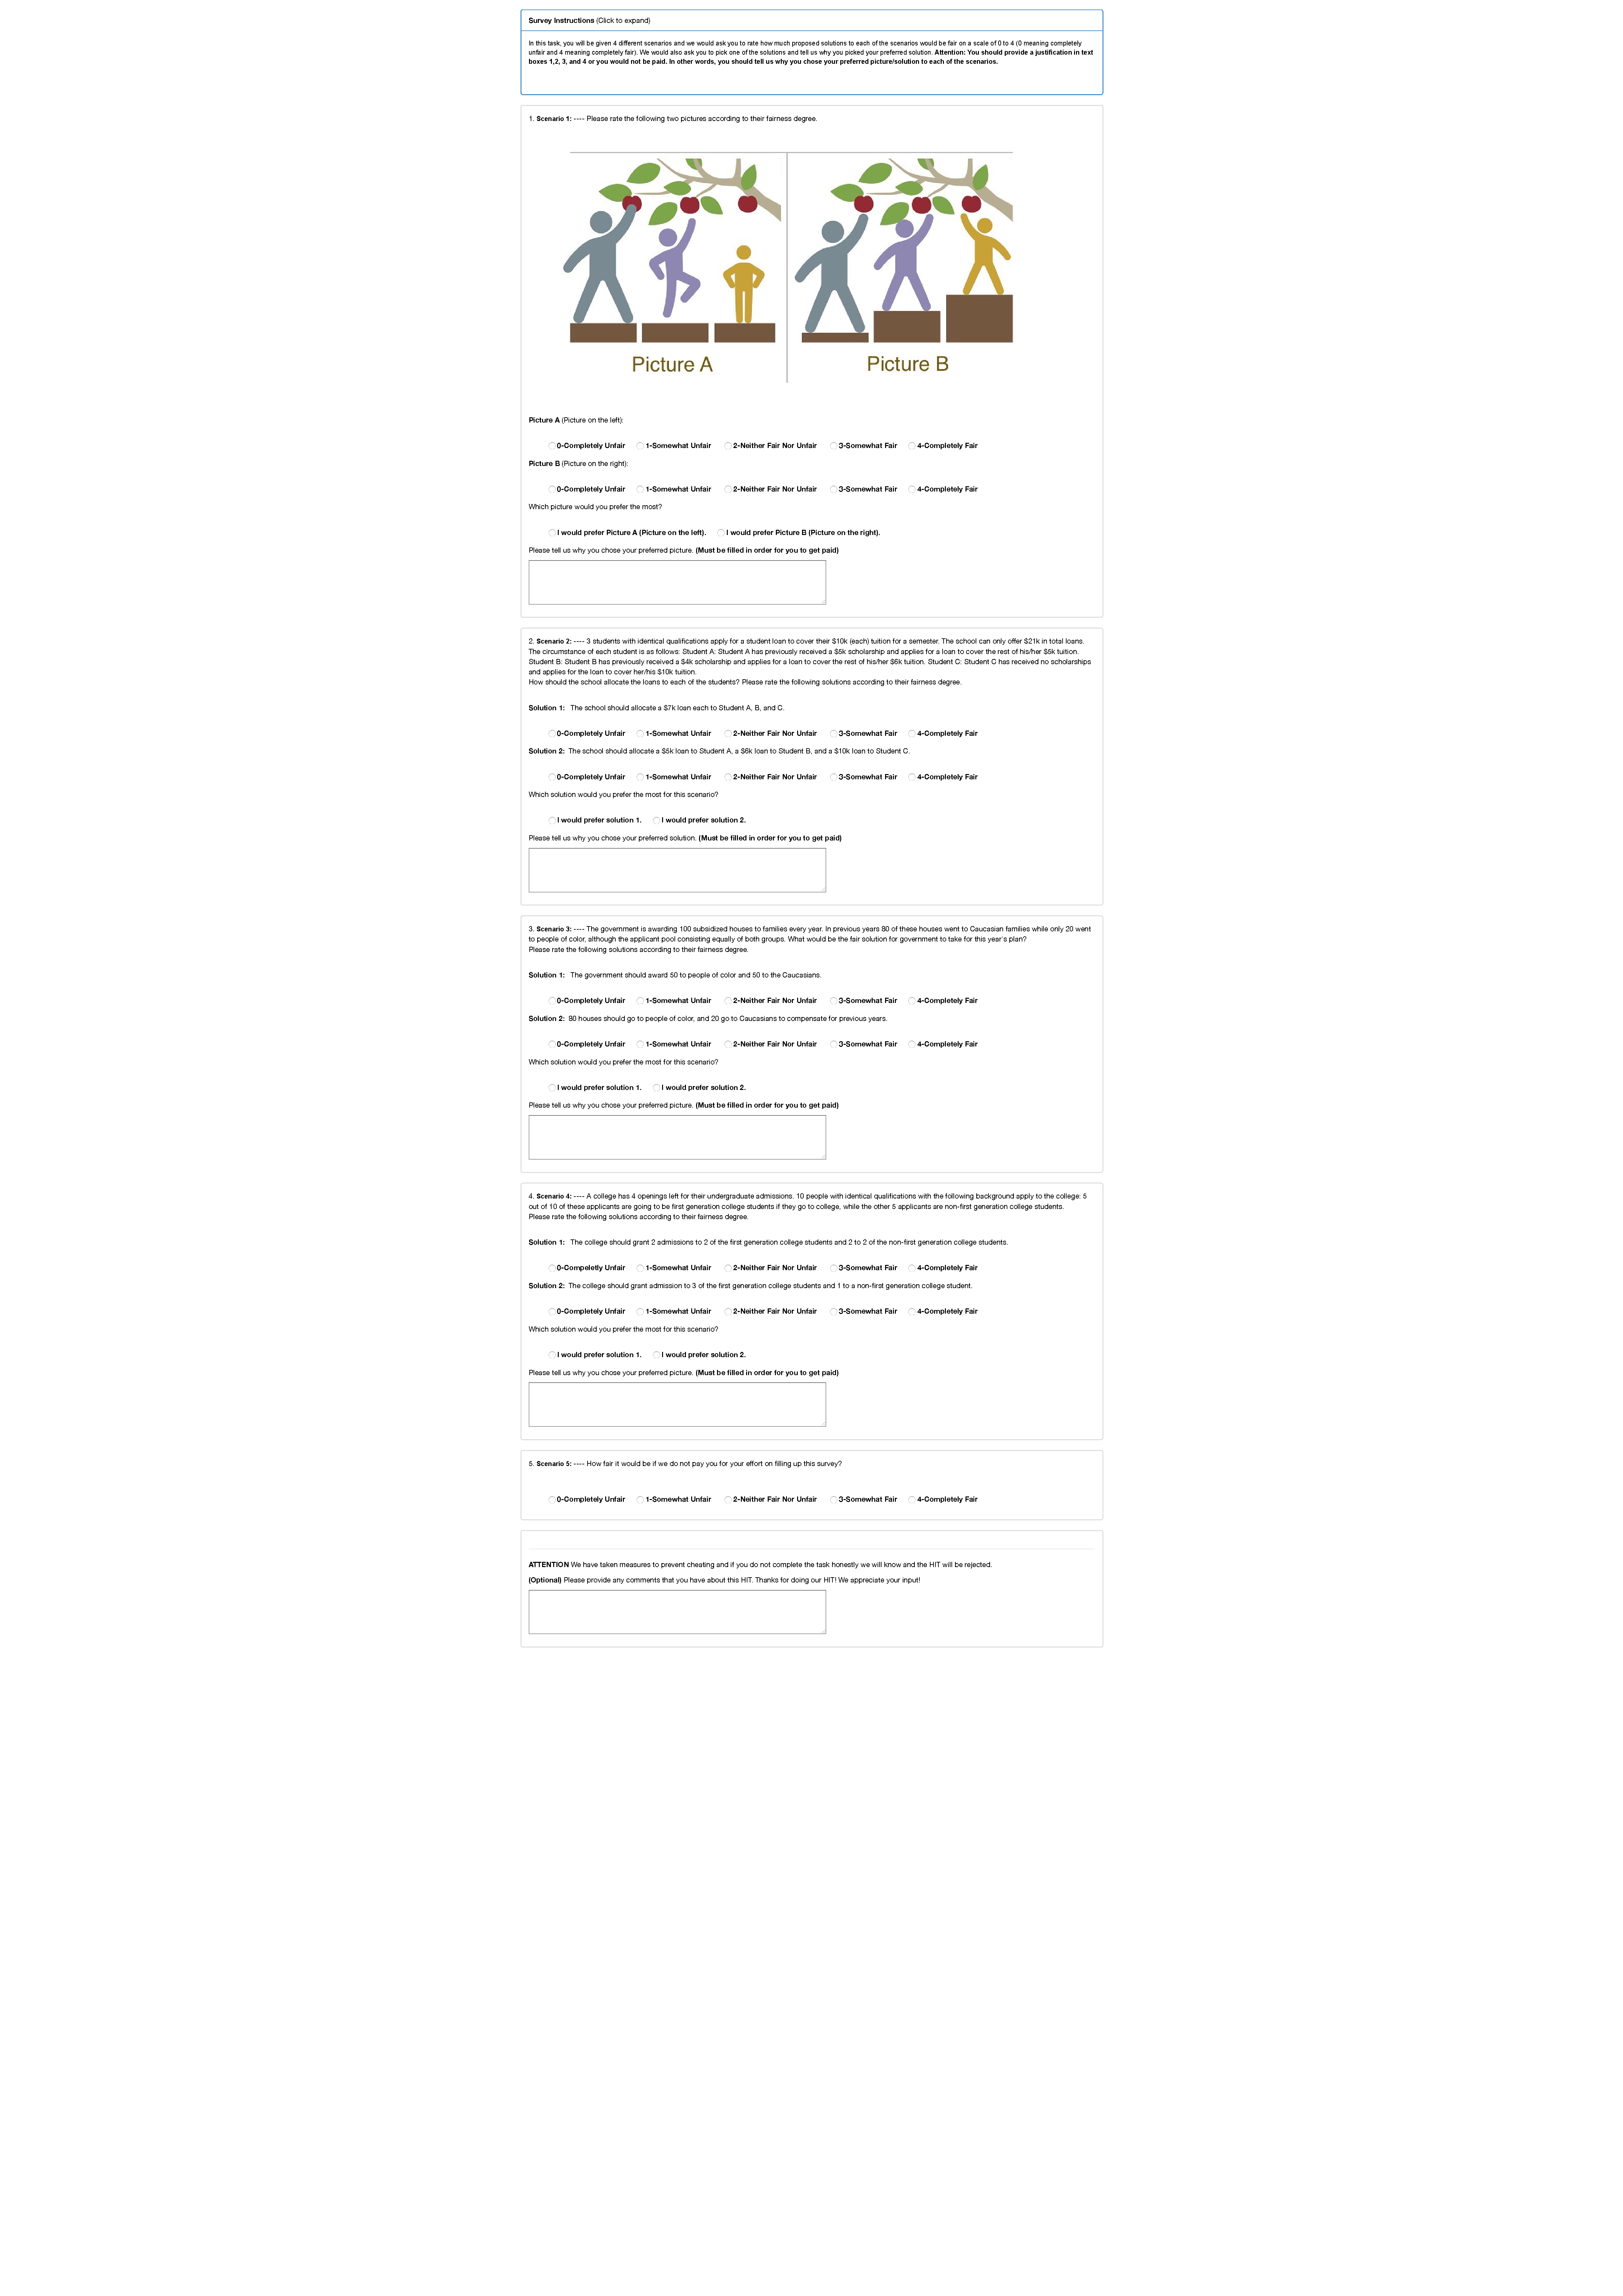
\includegraphics[width=0.5\textwidth,trim=26cm 33cm 26cm 0cm,clip=true]{images/small_survey.pdf}
\caption{Survey questionnaire used in the mechanical turk experiment.}
\label{survey}
\end{figure}

